\documentclass[12pt,a4paper]{article}
\usepackage[utf8]{inputenc}
\usepackage[german]{babel}
\usepackage{german}
\usepackage{hyperref,ulem,setspace}
\usepackage{graphicx}
\usepackage{caption}
\usepackage{subcaption}
\normalem

\title{Projektbericht}
\author{R. Brandis \and K. Läufer}
\date{\today}

\begin{document}
\maketitle
\newpage
\tableofcontents
\newpage

\section{Aufgabenstellung}

\section{Extern modulierter Laser}
Um mit einem mit konstanter Intensität strahlenden Laser Informationen zu übertragen, muss mindestens ein Parameter des Laserstrahls extern moduliert werden. Mögliche Modulationsparameter sind beispielsweise die Amplitude oder die Phase des Strahls. In unseren Versuchen kam ausschließlich Amplitudenmodulation zum Einsatz.

Wenn die Amplitude eines Laserstrahls extern moduliert werden soll, sind wiederum verschiedene Aufbauten als Modulatoren denkbar. Ein Lautsprecher mit einem in der Mitte der Membran angebrachten kleinen Spiegel kann je nach Auslenkung der Lautsprechermembran die Intensität des auf der Photodiode des Empfängers auftreffenden Lichts verändern; mit dieser Technik hat sich eine zweite Projektgruppe genauer beschäftigt. Wir haben uns stattdessen für die Variante entschieden, bei der ein einzelner LCD-Pixel (engl. liquid crystal display) zum Einsatz kommt.

\subsection{LCD-Modul als Modulator}
\begin{itemize}
\item Allgemeines Funktionsprinzip eines LCDs
\item Versuchsaufbau beschreiben
\item Resultate Übertragungsfunktion
\end{itemize}
Ein einzelner Pixel eines LCD besteht üblicherweise aus einer Flüssigkristallschicht, an die über zwei Elektroden ein elektrisches Feld angelegt werden kann, sowie einem horizontalen und einem vertikalen Polarisationsfilter, je einer vor und einer hinter der Kristallschicht.

Wären die Flüssigkristalle nicht vorhanden, würden beide Polarisationsfilter zusammen das gesamte einfallende Licht herausfiltern. Die zusätzliche Kristallschicht zwischen beiden Filtern sorgt nun für eine Drehung der Polarisation des durch den ersten Filter polarisierten Lichts. Da sich die Ausrichtung der Kristalle über das angelegte Feld bzw. über die angelegte Spannung steuern lässt, lässt sich somit auch die Menge des insgesamt durchgelassenen Lichts steuern.

Da in unserem Aufbau die Lichtquelle bereits polarisiertes Laserlicht aussendet, ist der erste Polarisationsfilter überflüssig.


\subsection{Übertragung von Audiosignalen}
\begin{itemize}
\item Aufbau erklären
\item Unterpunkt zu Lichtempfaengerschaltungen
\end{itemize}

\subsection{Übertragung digitaler Daten}





\section{Direkt modulierter Laser}
Im zweiten Teil des Projekts sollte ein Diodenlaser direkt moduliert werden um damit digitale Daten zu übertragen. Dazu hatte die andere Gruppe bereits eine Modulationsmethode untersucht, bei der auf einen konstanten Strom ein Datensignal aufgekoppelt wurde.

Unser Ziel war es eine Stromquelle direkt mit einem Datensignal zu modulieren und danach Empfängerdesigns zu evaluieren.


\subsection{Sender: modulierte Konstantstromquelle}
\label{sec:direct_tx}
Auf Grund der exponentiellen Kennlinie einer Laserdiode muss diese mit einem konstanten Strom versorgt werden. Eine einfache Konstantstromquelle kann mit zwei Bipolartransisoren aufgebaut werden. Der Strom $I_{D1}$ , der durch die Diode fließt entspricht hierbei in etwa dem Strom $I_{R1}$, der durch den Widerstand $R1$ fließt. An diesem müssen, durch den Transistor  $Q2$ vorgegeben, etwa $0.7V$ abfallen, wodurch sich ungefähr folgender Strom einstellt:

\begin{equation}
I_{D1} = I_{R1} = \frac{U_{R1}}{R1} \approx \frac{0.7V}{R1}
\end{equation}

Diese Quelle lässt sich leicht ein und aus schalten in dem - über einen Widerstand - die Kollektor-Emitter-Spannung $U_{CE2}$ des Transistor $Q2$ vorgegeben wird. Dieser Aufbau ist in Abbildung~\ref{fig:modulated_current_source} zu sehen.

\begin{figure}[h!]
  \centering
    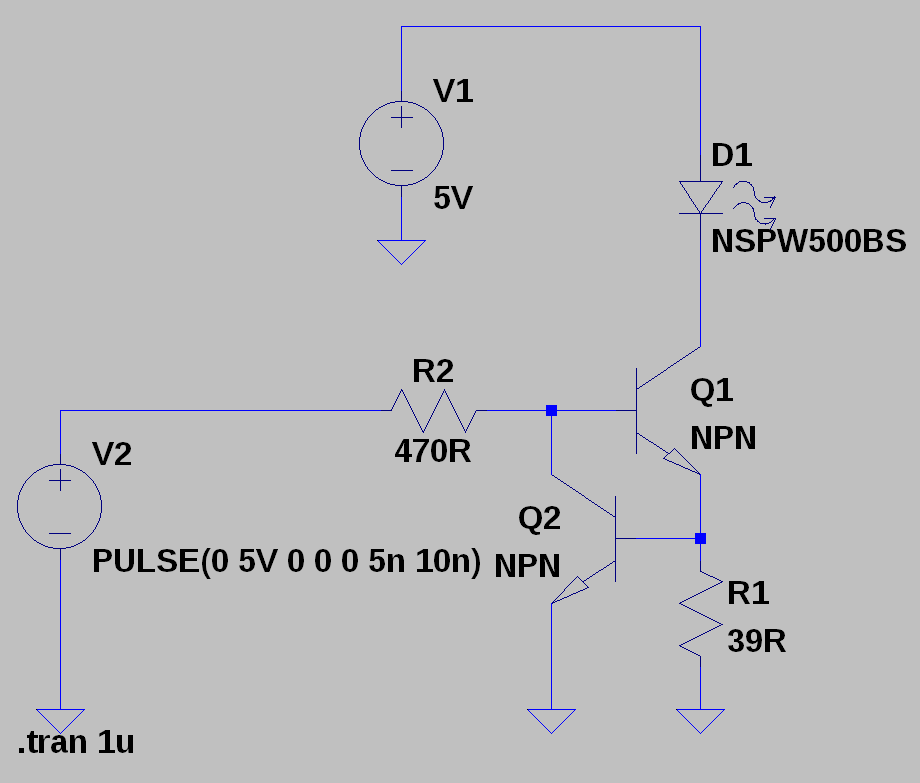
\includegraphics[width=0.8\textwidth]{../spice/modulated_current_source.png}
  \caption{Modulierte Stromquelle.}
  \label{fig:modulated_current_source}
\end{figure}

\begin{figure}[h!]
  \centering
    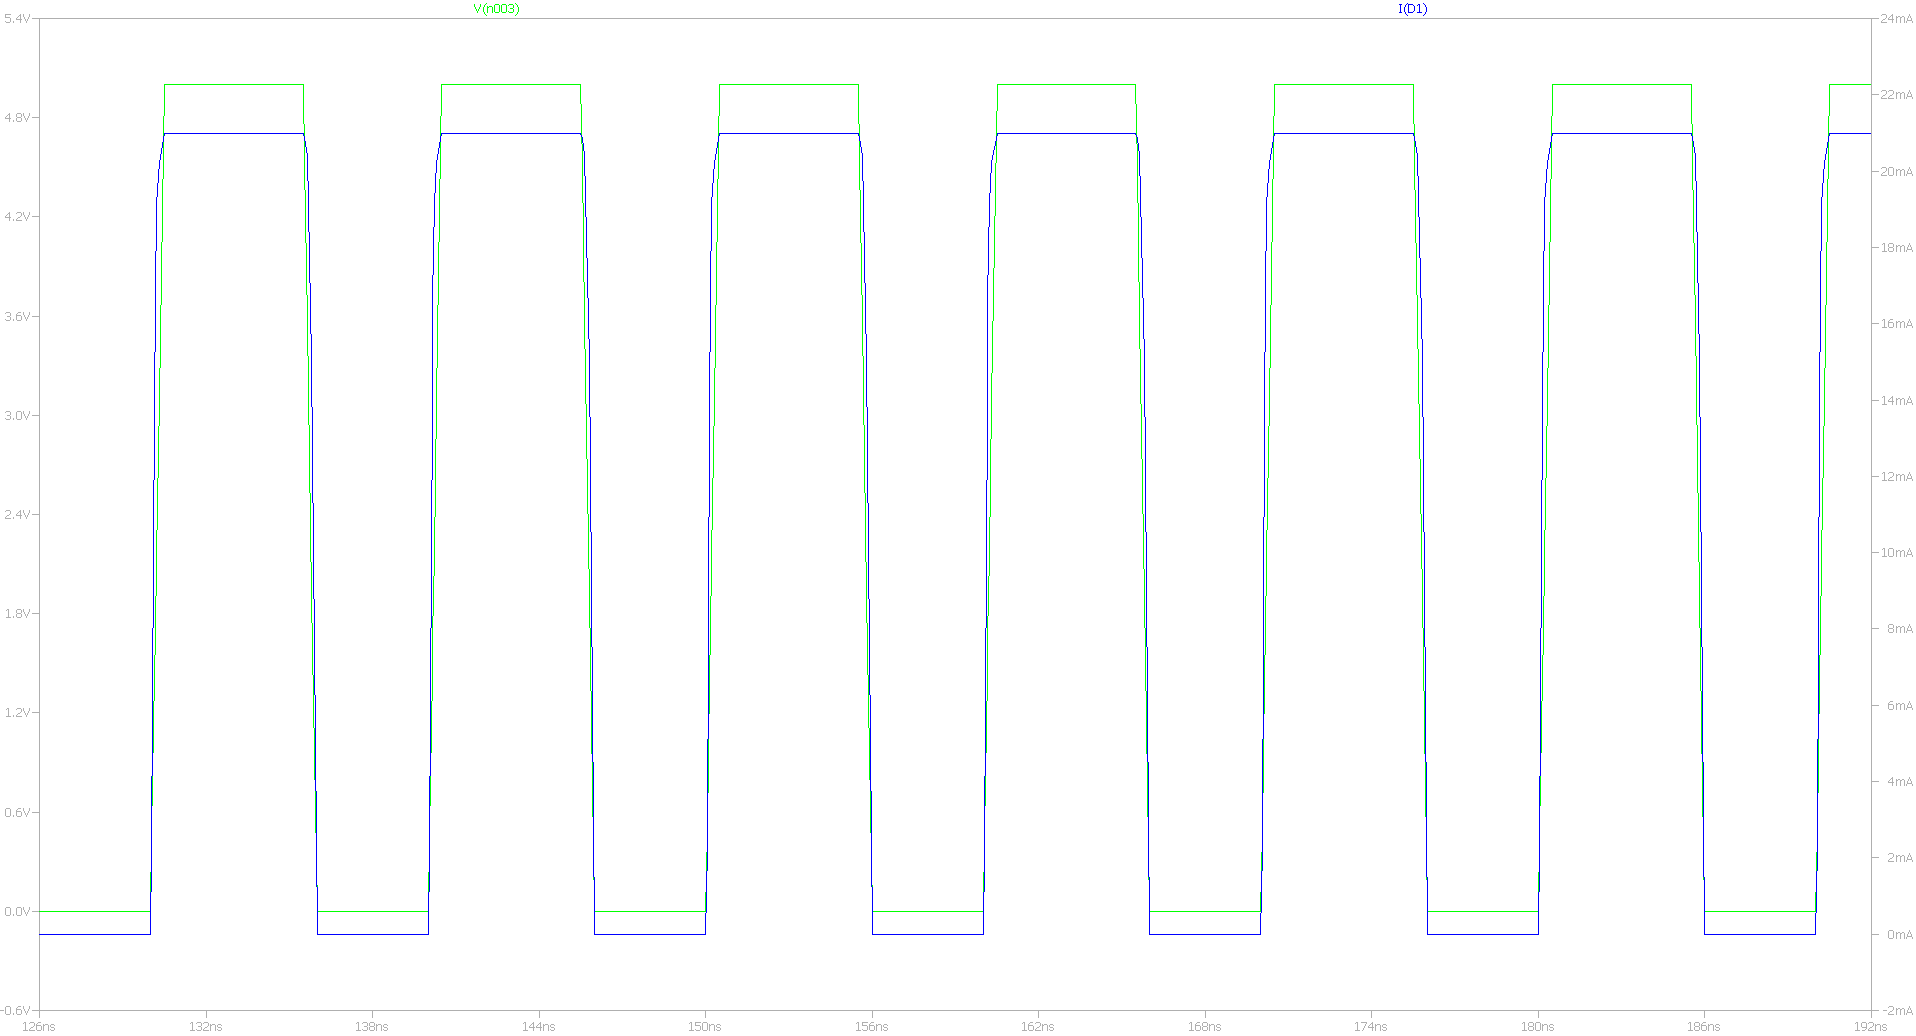
\includegraphics[width=1.0\textwidth]{../spice/current_input_v_current_out_trans.png}
  \caption{Transientenanalyse der modulierten Stromquelle.}
  \label{fig:modulated_current_source_plot}
\end{figure}


Eine Simulation des Aufbaus in LTSpice zeigt, dass der Strom $I_{D1}$ durch die Diode von der Eingangsspannung $U_2$ abhängt. Die in Abbildung~\ref{fig:modulated_current_source_plot} dargestellten Ergebnisse wurde aber mit einem vereinfachten Transistormodell simuliert, sind also mit Vorsicht zu genießen. Das Prinzip wird darin aber gut veranschaulicht.

\begin{figure}[h!]
  \centering
    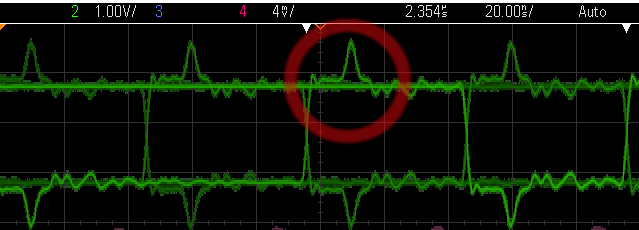
\includegraphics[width=1.0\textwidth]{img/ring_20MHz.png}
  \caption{Reflexionen bei einem $20MHz$ Eingangssignal.}
  \label{fig:ring_20mhz}
\end{figure}

Mit diesem Aufbau ließen sich recht schnelle Übertragungen von zufälligen Bits realisieren (siehe auch Abschnitt~\ref{sec:direct_rx}). Es gab jedoch, auf Grund der fehlenden Terminierung auf der Eingangsseite unserer Schaltung, Probleme mit Reflexionen auf der Leitung (siehe Abbildung~\ref{fig:ring_20mhz}). Hier wäre eine Untersuchung verschiedener Terminierungsvarianten interessant.

\subsection{Empfänger}
\label{sec:direct_rx}




\begin{itemize}
\item Schaltung erklären
\item Vergleich Ausgangspegel/Geschwindigkeit 10k Ohm vs 50 Ohm
\end{itemize}

\subsection{Augendiagramme}
Augendiagramme können mit dem Oszilloskop aufgenommen werden. Hierzu wird der Trigger auf steigende und fallende Flanken des Signals eingestellt und Persistenz aktiviert. Hierdurch erhält man eine Überlagerung von steigenden und fallenden Flanken. Verbleibt zwischen diesen eine klar erkennbare Öffnung (das Auge), dann kann man davon ausgehen, dass die Bits auch von einer Empfängerschaltung richtig interpretiert werden können. Wichtig ist, als Eingangssignal eine Zufallssequenz von Bits zu wählen, damit sich das System nicht einfach auf eine Frequenz einschwingt.

\begin{figure}[h!]
  \centering
    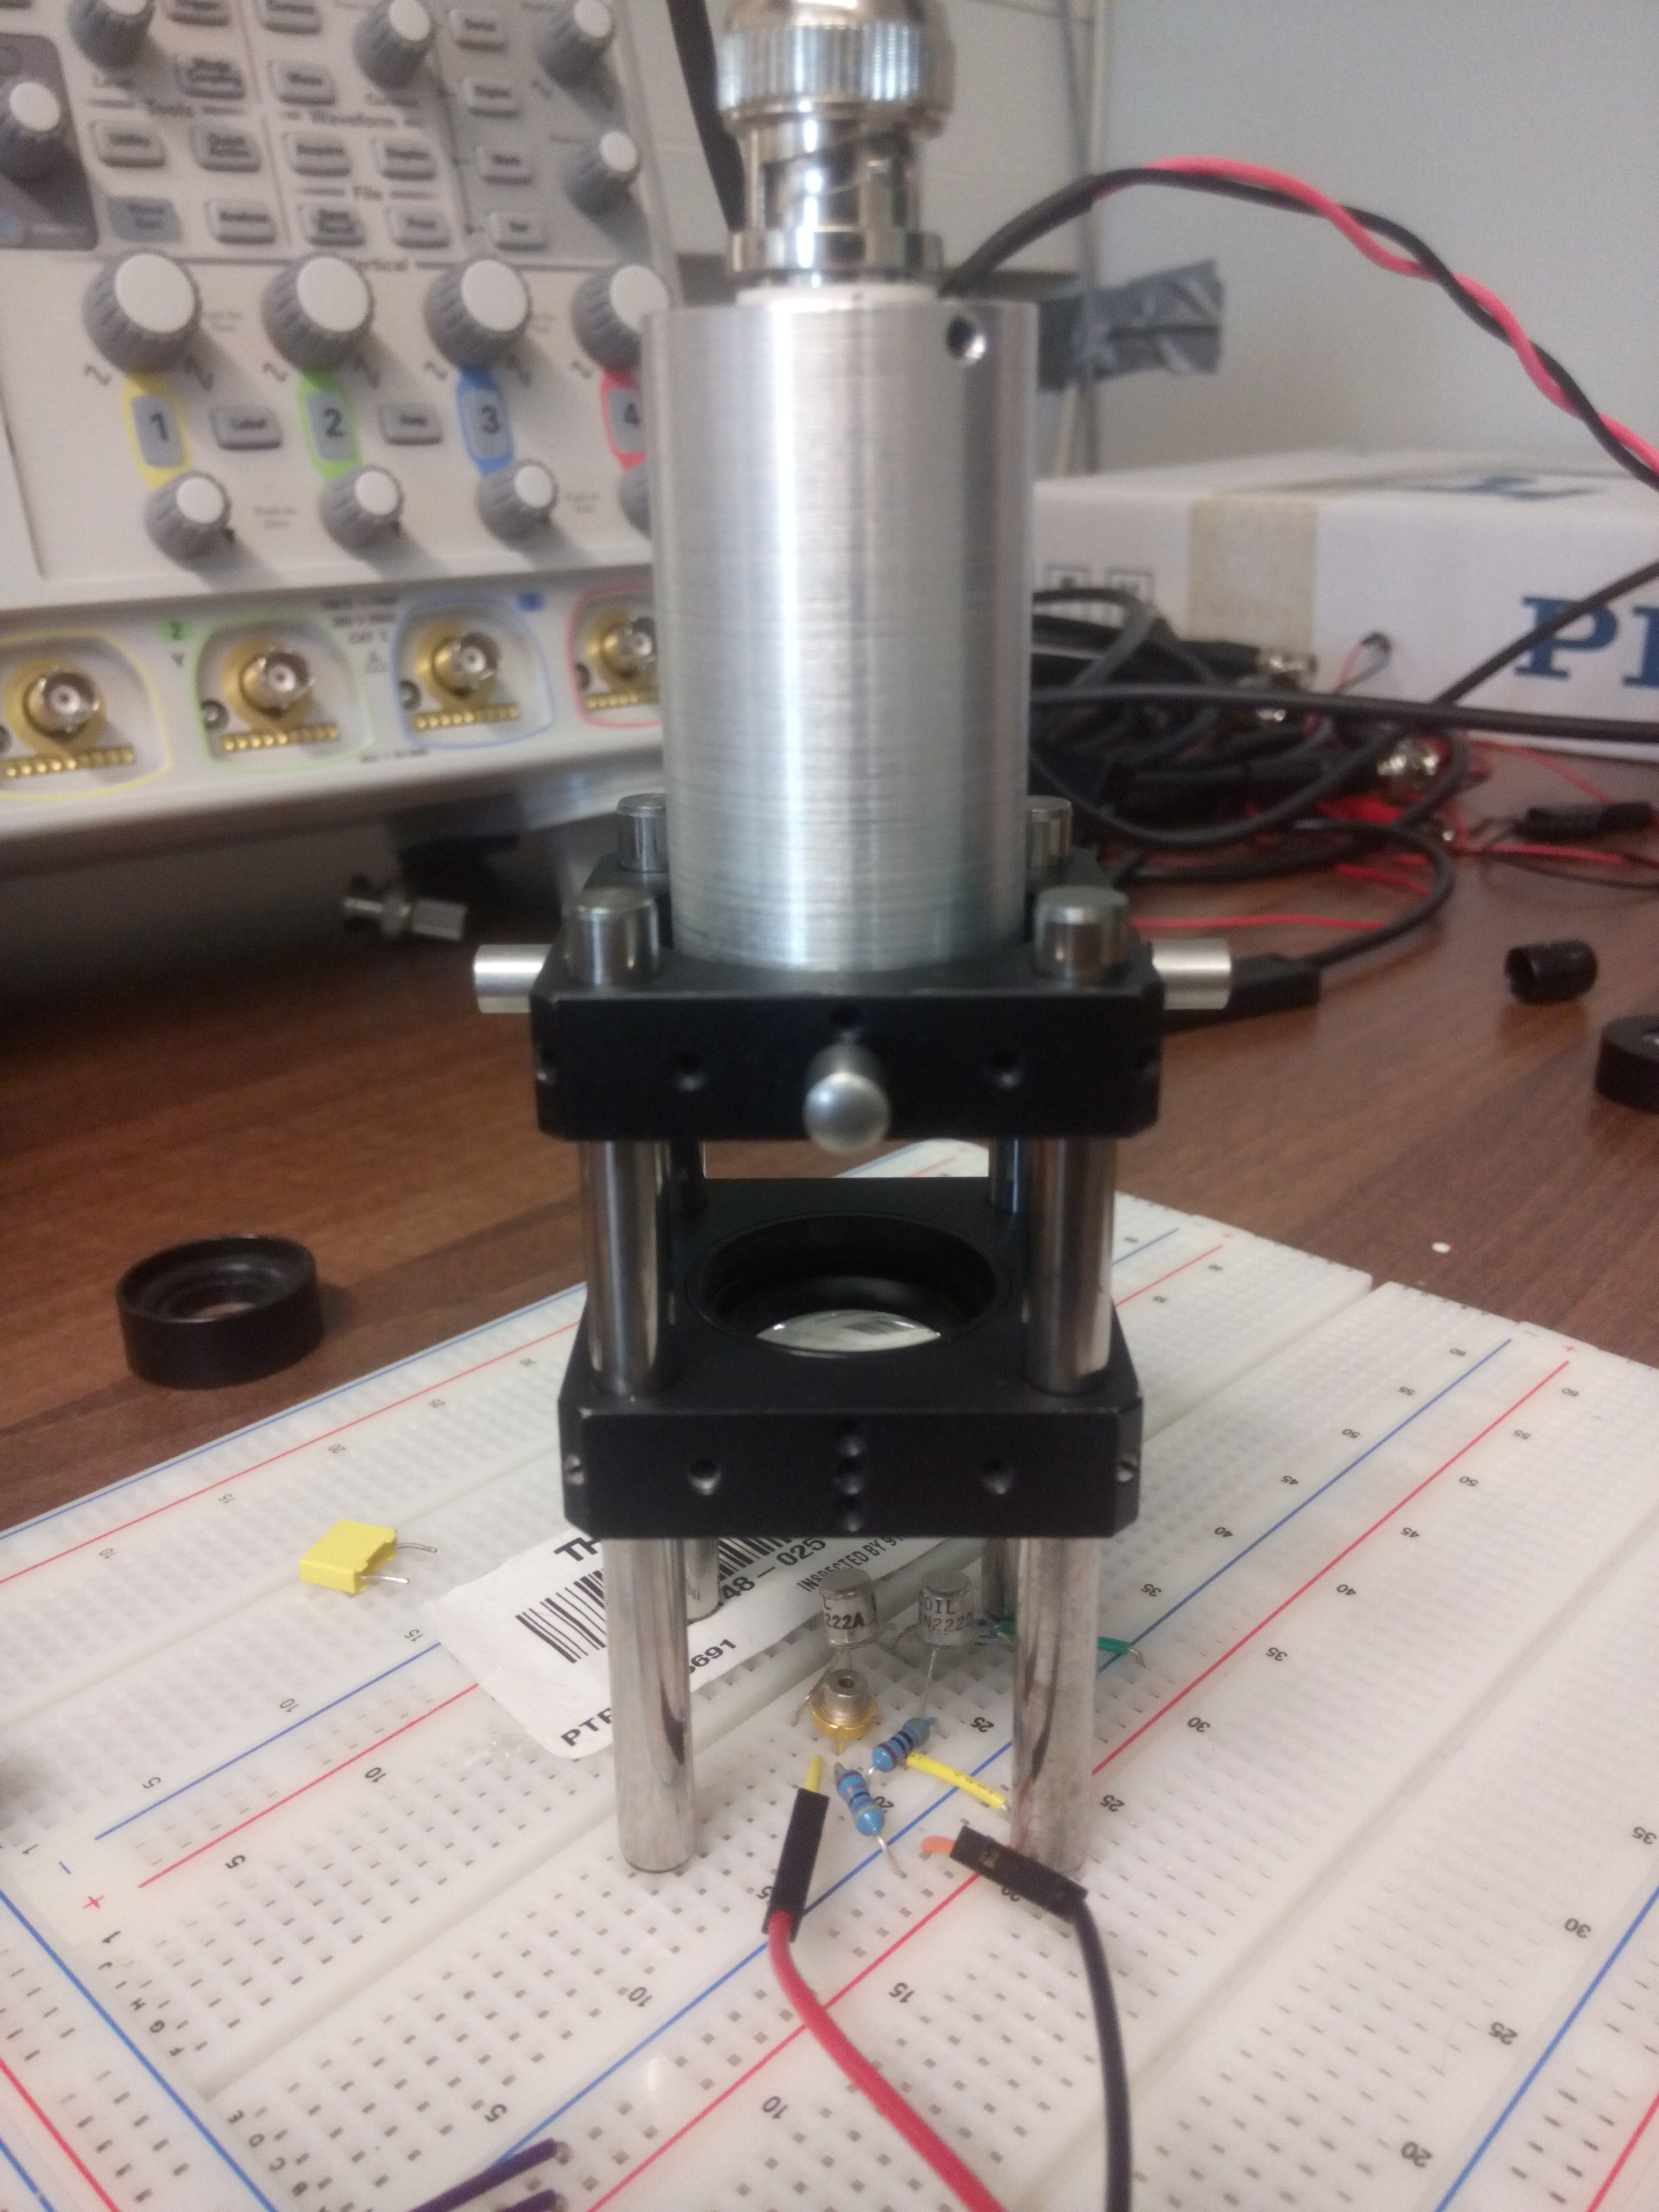
\includegraphics[width=0.7\textwidth]{../photos/IMG_20140710_184030.jpg}
  \caption{Versuchsaufbau zur Bestimmung der Augendiagramme.}
  \label{fig:eye_setup}
\end{figure}

\begin{figure}
  \centering
  \begin{subfigure}[b]{0.6\textwidth}
    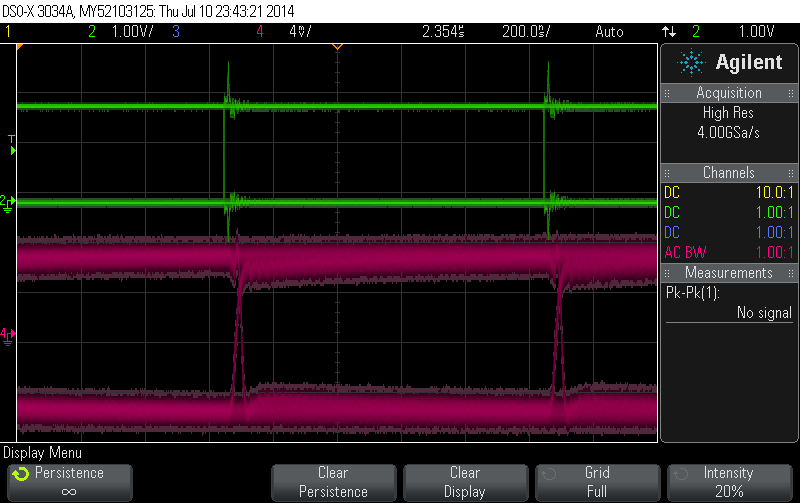
\includegraphics[width=\textwidth]{../measurements/20140710/eye_plots/01MHz.png}
    \caption{$1MHz$}
  \end{subfigure}  
  \begin{subfigure}[b]{0.6\textwidth}
    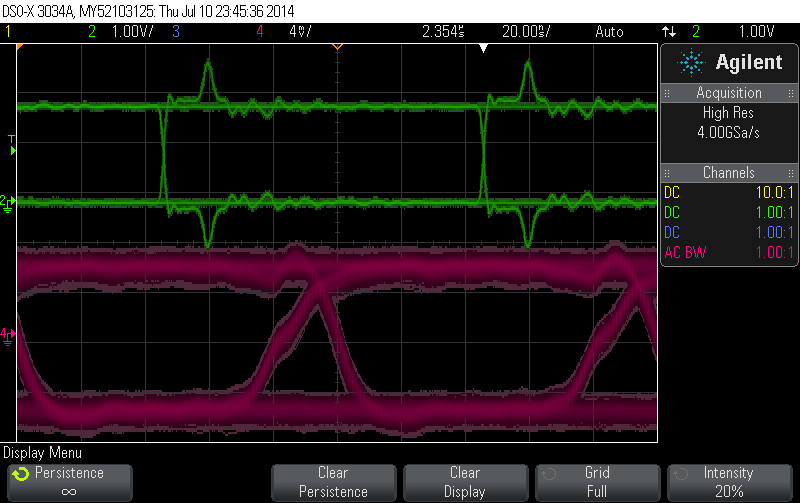
\includegraphics[width=\textwidth]{../measurements/20140710/eye_plots/10MHz.png}
    \caption{$10MHz$}
  \end{subfigure}  
  \begin{subfigure}[b]{0.6\textwidth}
    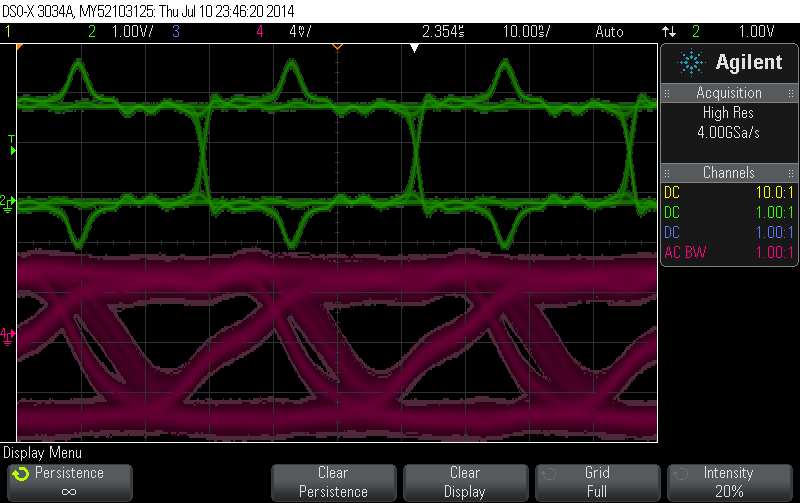
\includegraphics[width=\textwidth]{../measurements/20140710/eye_plots/30MHz.png}
    \caption{$30MHz$}
  \end{subfigure}  
  \begin{subfigure}[b]{0.6\textwidth}
    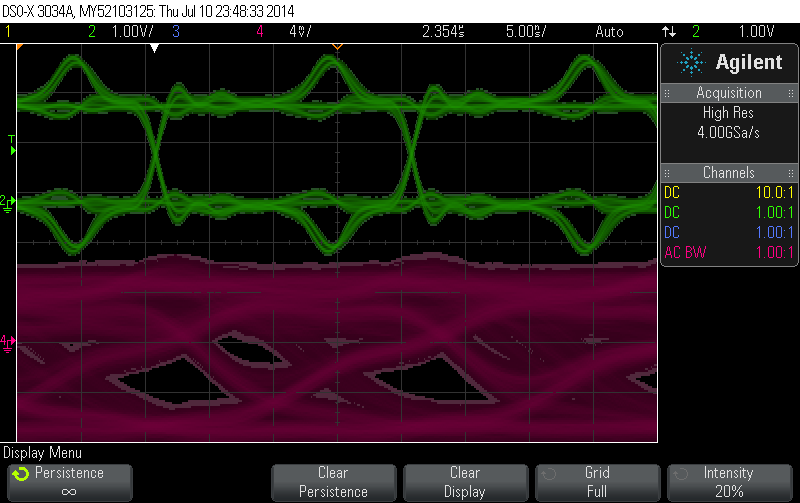
\includegraphics[width=\textwidth]{../measurements/20140710/eye_plots/50MHz.png}
    \caption{$50MHz$}
  \end{subfigure}  
  \caption{Augendiagramme}
  \label{fig:eye_plots}
\end{figure}

In unserem Fall wurden die Augendiagramme in Abbildung~\ref{fig:eye_plots} mit der Sendeschaltung aus Abschnitt~\ref{sec:direct_tx} und der Empfängerschaltung mit dem \textit{AD8015} TIA aufgenommen. Der Aufbau ist in Abbildung~\ref{fig:eye_setup} zu sehen.

Ein $1MHz$ Bitsignal wird ohne Probleme übertragen, auch bei einem $10MHz$ Signal ist die Augenöffnung noch unproblematisch. Ein $30MHz$ Signal hat bereits eine deutlich kleiner Öffnung, sollte aber auch noch funktionieren. Bei einem $50MHz$ Signal scheint die Grenze erreicht; hier ist keine distinkte Öffnung mehr zu erkennen. 

\begin{itemize}
\item Vergleich Photodiode und integrierter Transimpedanzverstärker
\item Besprechen der Resultate
\end{itemize}

\section{Fazit}

\end{document}
